\chapter{Complex integration}

\section{Complex integrals of real-valued functions}

\begin{definition}
    \label{def:complex-integral-real-variable}
    Let \(f: [a, b] \subseteq \R \to \C\) be a complex-valued function of a real variable \(t\). Then the definite integral of \(f\) over \([a, b]\) is defined as
    \begin{equation}
        \int_a^b f(t) \, dt = \int_a^b u(t) \, dt + i \int_a^b v(t) \, dt,
        \label{eq:complex-integral-real-variable}
    \end{equation}
    where \(f(t) = u(t) + iv(t)\) with \(u\) and \(v\) continuous for all \(t \in [a, b]\).
\end{definition}

It follows immediately from Definition~\ref{def:complex-integral-real-variable} that
\[
    \Re \int_a^b f(t) \, dt = \int_a^b u(t) \, dt = \int_a^b \Re f(t) \, dt
\]
and
\[
    \Im \int_a^b f(t) \, dt = \int_a^b v(t) \, dt = \int_a^b \Im f(t) \, dt.
\]

If \(U\) and \(V\) are antiderivatives of \(u\) and \(v\) respectively, then the integral in \eqref{eq:complex-integral-real-variable} of \(f\) over \([a, b]\) can be written as
\[
    \int_a^b f(t) \, dt = [U(t) + iV(t)]\big|_a^b = U(b) - U(a) + i[V(b) - V(a)].
\]

\begin{example}
    Evaluate the integral
    \[
        \int_0^1 (t-i)^3 \, dt.
    \]
    \begin{solution}
        We write the integrand in terms of real and imaginary parts:
        \begin{align*}
            (t - i)^3 &= t^3 - 3it^2 - 3t + i \\
            &= t^3 - 3t + i(-3t^2 + 1).
        \end{align*}
        Thus from Definition~\ref{def:complex-integral-real-variable}, we have
        \begin{align*}
            \int_0^1 (t - i)^3 \, dt &= \int_0^1 t^3 - 3t \, dt + i \int_0^1 -3t^2 + 1 \, dt \\
            &= \left[ \frac{t^4}{4} - \frac{3t^2}{2} \right]_0^1 + i \left[ -t^3 + t \right]_0^1 \\
            &= \frac{1}{4} - \frac{3}{2} + i(-1 + 1) = -\frac{5}{4}.
        \end{align*}
    \end{solution}
\end{example}

\begin{example}
    \label{ex:complex-integral-real-variable-exp-t-it}
    Evaluate \(\displaystyle\int_0^{\pi/2} \exp(t + it) \, dt\).
    \begin{solution}
        We have
        \begin{align*}
            \int_0^{\pi/2} \exp(t + it) \, dt &= \int_0^{\pi/2} e^t e^{it} \, dt \\
            &= \int_0^{\pi/2} e^t (\cos t + i \sin t) \, dt \\
            &= \int_0^{\pi/2} e^t\cos t \, dt + i \int_0^1 e^t \sin t \, dt.
        \end{align*}

        Now we can integrate by parts to get
        \begin{align*}
            \int_0^{\pi/2} \underbrace{e^t}_{u} \underbrace{\cos t \, dt}_{dv} &= \underbrace{e^t}_{u} \underbrace{\sin t}_{v} \bigg|_0^{\pi/2} - \int_0^{\pi/2} \underbrace{\sin t}_{v} \underbrace{e^t \, dt}_{du} \\
            &= (e^{\pi/2} \sin \frac{\pi}{2} - e^0 \sin 0) - \int_0^{\pi/2} e^t \sin t \, dt.\\
            &= (e^{\pi/2} ) - \int_0^{\pi/2} e^t \sin t \, dt.\\
            &= e^{\pi/2} - \int_0^{\pi/2} \underbrace{e^t}_{u} \underbrace{\sin t \, dt}_{dv} \\
            &= e^{\pi/2} - (\underbrace{e^t}_{u} \underbrace{-\cos t}_{v}) \bigg|_0^{\pi/2} + \int_0^{\pi/2} \underbrace{-\cos t}_{v}~\underbrace{e^t \, dt}_{du} \\
            &= e^{\pi/2} - 1 - \int_0^{\pi/2} e^t \cos t \, dt.
        \end{align*}
        Adding the integral \(\int_0^{\pi/2} e^t \cos t\, date\) to both sides and dividing by \(2\) gives
        \[
            \int_0^{\pi/2} e^t \cos t \, dt = \frac{e^{\pi/2} - 1}{2}.
        \]
        Similarly,
        \[
            \int_0^{\pi/2} e^t \sin t \, dt = \frac{i}{2}(e^{\pi/2} + 1).
        \]
        Applying the definition thus yields
        \[
            \int_0^{\pi/2} \exp(t + it) \, dt = \frac{e^{\pi/2} - 1}{2} + \frac{i}{2}(e^{\pi/2} + 1).
        \]
    \end{solution}
\end{example}

We quickly validate some rules of integration from calculus.

\begin{theorem}
    Let \(f\) and \(g\) be complex-valued functions of a real variable \(t\) and let \(z_0\) be a complex constant. Then
    \begin{enumerate}[label=(\alph*)]
        \item \(\displaystyle \int_a^b z_0 f(t) \, dt = z_0 \int_a^b f(t) \, dt\),
        \item \(\displaystyle \int_a^b \left( f(t) + g(t) \right) \, dt = \int_a^b f(t) \, dt + \int_a^b g(t) \, dt\),
        \item \(\displaystyle \int_a^b f(t) \, dt = -\int_b^a f(t) \, dt\).
        \item \(\displaystyle \int_a^b f(t) \, dt = \int_a^c f(t) \, dt + \int_c^b f(t) \, dt\).
    \end{enumerate}
\end{theorem}

We also restate the fundamental theorem of calculus.

\begin{theorem}[Fundamental theorem of calculus (real-variable)]
    \label{thm:fundamental-theorem-calculus-real-variable}
    Let \(f\) be a continuous function on \([a, b]\) and let \(F\) be a function such that \(F'(t) = f(t)\) for all \(t \in [a, b]\). Then
    \begin{equation}
        \int_a^b f(t) \, dt = F(b) - F(a).
        \label{eq:fundamental-theorem-calculus-real-variable}
    \end{equation}
\end{theorem}

Some important results from real-variable calculus, however, do not carry over to complex-valued functions of a real variable. As we shall see in the following two examples.

\begin{example}
    Show that the mean-value theorem for derivatives does not generally hold for complex-valued functions of a real variable.

    \begin{solution}
        The mean-value theorem for derivatives states that if \(f\) is continuous and differentiable on \([a, b]\), then there exists a \(c \in (a, b)\) such that
        \[
            f'(c) = \frac{f(b) - f(a)}{b-a}.
        \]
        Consider the function \(f(t) = e^{it}\) on the interval \([0, 2\pi]\). Its derivative is \(f'(t) = ie^{it}\) and so for any \(c \in (0, 2\pi)\), we have
        \[
            |f'(c)| = |ie^{ic}| = 1,
        \]
        so that \(f'(t)\) is never zero. However, \(f(2\pi) - f(0) = 0\).
    \end{solution}
\end{example}

\begin{example}
    Show that the mean-value theorem for integrals does not generally hold for functions of the form \(f(t) = u(t) + iv(t)\).

    \begin{solution}
        Consider the function \(f(t) = e^{it}\) on the interval \([0, 2\pi]\). Then
        \[
            \int_0^{2\pi} e^{it} \, dt = \left. \frac{e^{it}}{i} \right|_0^{2\pi} = 0.
        \]

        Now recall that the mean-value theorem for integrals states that if \(f\) is continuous and integrable on \([a, b]\), then there exists a \(c \in [a, b]\) such that
        \[
            f(c) = \frac{1}{b-a} \int_a^b f(t) \, dt
        \]
        so that,
        \[
            \int_a^b f(t) \, dt = f(c)(b-a).
        \]

        However for any \(c \in [0, 2\pi]\), we have
        \[
            |e^{ic}(2\pi - 0) | = 2\pi \neq 0
        \]
        and thus \(f(c)(b - a) \neq \int_a^b f(t) \, dt\) and the mean-value theorem for integrals does not hold for complex-valued functions of a real variable.
    \end{solution}
\end{example}

\begin{example}
    Use Equation~\eqref{eq:fundamental-theorem-calculus-real-variable} to evaluate the integral in Example~\ref{ex:complex-integral-real-variable-exp-t-it}.

    \begin{solution}
        We need to find a function \(F\) such that \(F'(t) = exp(t + it)\). Observe that
        \[
            F(t) = \frac{1}{1 + i} e^{t + it}
        \]
        satisfies this condition. Thus by Equation~\eqref{eq:fundamental-theorem-calculus-real-variable}, we have
        \begin{align*}
            \int_0^{\pi/2} \exp(t + it) \, dt &= \frac{1}{1 + i} e^{t + it} \bigg|_0^{\pi/2} \\
            &= \frac{1}{1 + i} (ie^{\pi/2} - e^0) \\
            &= \frac{1}{2} (1 - i)(ie^{\pi/2} - 1) \\
            &= \frac{1}{2} (e^{\pi/2} - 1) + \frac{i}{2} (e^{\pi/2} + 1).
        \end{align*}
        This agrees with the result obtained in Example~\ref{ex:complex-integral-real-variable-exp-t-it}.
    \end{solution}
\end{example}

\section{Contour integrals}

\begin{definition}
    An \emph{arc} (or a \emph{curve}) \(\gamma\) on the complex plane is the
    image of a continuous function \(\gamma : [a, b] \to \C\), where \(a, b \in
    \R\), that is,
    \[
        \gamma = \{\gamma(t) : a \leq t \leq b\}.
    \]
\end{definition}

It would be more convenient to write
\[
    z = z(t) = x(t) + iy(t),
\]
where \(x(t)\) and \(y(t)\) are continuous functions of \(t\), so that
\[
    z = \gamma(t).
\]

We call \(z(t)\) a \emph{parametrization} of the arc \(\gamma\). The points
\emph{a} and \emph{b} are the \emph{initial} and \emph{terminal} points of the
arc \(\gamma\), respectively. The \emph{opposite arc} \(-\gamma\) is the arc
\(\gamma\) traversed in the opposite direction, i.e., from \emph{b} to \emph{a}.

\begin{theorem}
    An arc is compact and connected.
\end{theorem}

\begin{proof}
    Since \([a, b] \subseteq \R\) is closed and bounded, it is compact. Since
    \(\gamma\) is continuous, it follows that \(\gamma([a, b])\) which is a
    continuous image of a compact set is also compact. Similarly, since the
    continuous image of a connected set is connected, it follows that
    \(\gamma([a, b])\) is connected.
\end{proof}

\begin{example}
    Find a parametrization of the arcs \(\gamma\) and \(-\gamma\), where
    \(\gamma\) is the straight line from the point \(z_0 = (x_0, y_0)\) to the
    point \(z_1 = (x_1, y_1)\).

    \begin{solution}
        From calculus, we know that the line in \(\R^2\) from \(z_0\) to \(z_1\)
        is given by the vector \(z_1 - z_0\). Thus a parametrization of the line
        is given by
        \begin{align*}
            z(t) &= z_0 + t(z_1 - z_0) \\
            &= (x_0, y_0) + t[(x_1 - x_0) + i(y_1 - y_0)] \\
            &= (x_0 + t(x_1 - x_0), y_0 + t(y_1 - y_0)),
        \end{align*}
        for \(0 \leq t \leq 1\). Similarly, a parametrization of the opposite arc \(-\gamma\) is given by
        \[
            z^*(t) = z_1 + t(z_0 - z_1) = (x_1 + t(x_0 - x_1), y_1 + t(y_0 - y_1)),
        \]
        for \(0 \leq t \leq 1\).

        In general, we can see that if \(z(t)\) is a parametrization of
        \(\gamma\), then \(z^*(t) = z(b + a - t)\) is a parametrization of
        \(-\gamma\). (In particular, if \(a = 0\) and \(b = 1\), then \(z^*(t) =
        z(1 - t)\).)
    \end{solution}
\end{example}


Some additional definitions are in order.

\begin{definition}
    An arc \(\gamma\) is \emph{simple} if it does not intersect itself, i.e., if
    \(\gamma(t_1) = \gamma(t_2)\) implies \(t_1 = t_2\). An arc \(\gamma\) is
    \emph{closed} if \(\gamma(a) = \gamma(b)\). An arc \(\gamma\) that is both
    simple and closed is a \emph{simple closed curve} (or a \emph{Jordan
    curve}).

    An arc \(\gamma\) is \emph{smooth} if its parametrization \(z(t)\) is
    continuously differentiable and \(z'(t) \neq 0\) for all \(t \in [a, b]\). A
    \emph{contour} is a piecewise smooth arc, i.e., an arc that is the union of
    a finite number of smooth arcs.
\end{definition}


\begin{definition}
    Let \(\gamma\) be a contour with the equation \(z = z(t)\) for \(a \leq t
    \leq b\) contained in some region \(\Omega\) and let \(f\) be a function
    defined and continuous on \(\gamma\). Then the integral of \(f\) along
    \(\gamma\) is defined as
    \[
        \int_\gamma f(z) \, dz = \int_a^b f(z(t)) z'(t) \, dt.
    \]
    \label{def:complex-integral-contour}
\end{definition}

If the contour \(\gamma\) is a positively-oriented simple closed curve, then we write
\[
    \oint_\gamma f(z) \, dz
\]
to emphasize that the integration is along a closed curve.

\begin{example}
    \label{ex:complex-integral-contour-different-paths}
    Whereas the integral of functions of a real variable (whether real-valued or
    complex-valued) depends only on the endpoints of the interval of
    integration, the integral of a function of a complex variable along a
    contour depends on the path taken by the contour as
    Definition~\ref{def:complex-integral-contour} clearly indicates that the
    integration is defined along some contour \(\gamma\). This important because
    while there is a unique way to go from a point \(a\) to a point \(b\) in the
    real line, there are infinitely many ways to go from a point \(a\) to a
    point \(b\) in the complex plane.
    
    To belabor this point, consider the function \(f : \C \to \C\) defined by
    \(f(z) = \conj{z}^2\) along several paths from \(0\) to \(1 + i\). 
    \begin{enumerate}[label=(\alph*), wide, nosep]
        \item In the first case, let \(\gamma\) be the line segment from \(0\)
        to \(1 + i\). A parametrization of this path is given by \(z(t) = t(1 +
        i) = t + it\) for \(0 \leq t \leq 1\). Thus since \(z'(t) = 1 + i\) and
        \(f(z(t)) = \conj{t + it}^2 = (t - it)^2\), the integral of \(f\) along
        \(\gamma\) is
        \[
            \begin{aligned}
                \int_\gamma f(z) \, dz &= \int_0^1 (t - it)^2 (1 + i) \, dt \\
                &= (1 + i) \int_0^1 (1 - i)^2 t^2 \, dt \\
                &= (1 + i)(1 - i)^2 \int_0^1 t^2 \, dt \\
                &= (2 - 2i) \left[ \frac{t^3}{3} \right]_0^1 \\
                &= \frac{2}{3}(1 - i).
            \end{aligned}
        \]

        \item If \(\gamma\) is the arc of the parabola \(y = x^2\) from \(0\) to
        \(1 + i\), then a parametrization of this path is given by \(z(t) = t +
        it^2\) for \(0 \leq t \leq 1\). Then \(z'(t) = 1 + 2it\) and
        \[
            f(z(t)) = \conj{t + it^2}^2 = (t - it^2)^2 = t^2 - t^4 - 2it^3,
        \]
        so that the integral of \(f\) along \(\gamma\) is
        \[
            \begin{aligned}
                \int_\gamma f(z) \, dz &= \int_0^1 (t^2 - t^4 - 2it^3)(1 + 2it) \, dt \\
                &= \int_0^1 (t^2 + 3t^4 - 2it^5) \, dt \\
                &= \frac{14}{15} - \frac{i}{3}.
            \end{aligned}
        \]
    \end{enumerate}
    We have thus seen that the integral of \(f\) along \(\gamma\) depends on the
    path taken by \(\gamma\) and not just the endpoints of the path.
\end{example}

On the other hand, given a curve \(\gamma\), the following result tells us that
the actual choice of parametrization does not affect the value of the integral.

\begin{theorem}[Invariance under reparametrization]
    Let \(\gamma\) be a contour with the equation \(z = z(t)\) for \(a \leq t
    \leq b\) and let \(\phi: [\alpha, \beta] \to [a, b]\) be a reparametrization
    of \(\gamma\). Then
    \[
        \int_\gamma f(z) \, dz = \int_{\phi(\gamma)} f(z) \, dz.
    \]
\end{theorem}

\begin{proof}
    For all \(\tau \in [\alpha, \beta]\), we can find a unique \(t \in [a, b]\) such that \(t = \phi(\tau)\). Then if \(\zeta(\tau)\) is another parametrization of \(\gamma\), we have
    \[
        \zeta(\tau) = z(\phi(\tau)) = z(t).
    \]
    Differentiating with respect to \(\tau\) gives
    \[
        \zeta'(\tau) = \left( z(\phi(\tau)) \right)' = z'(\phi(\tau)) \phi'(\tau).
    \]
    Now from the definition of the integral along \(\gamma\), we have
    \begin{align*}
        \int_{\phi(\gamma)} f(z) \, dz &= \int_{\phi(\alpha)}^{\phi(\beta)} f(\zeta(\tau)) \zeta'(\tau) \, d\tau \\
        &= \int_{\phi(\alpha)}^{\phi(\beta)} f(z(\phi(\tau))) z'(\phi(\tau)) \phi'(\tau) \, d\tau \\
        &= \int_{a}^{b} f(z(t)) z'(t) \, dt\\
        &= \int_{\gamma} f(z) \, dz.
    \end{align*}
\end{proof}

We note that while Example \ref{ex:complex-integral-contour-different-paths}
shows that the integral of a function of a complex variable along a contour
depends on the path taken by the contour, the invariance under reparametrization
tells us that the actual choice of parametrization does not affect the value of
the integral. That is, since all parametrizations of a contour \(\gamma\) are
equivalent, the integral of a function of a complex variable along \(\gamma\) is
well-defined. In Example \ref{ex:complex-integral-contour-different-paths}, we
are talking about different contours altogether, not different parametrizations
of the same contour.

A related result tells us that a change in the orientation of the contour
changes the sign of the integral.

\begin{theorem}
    Let \(\gamma\) be a contour with the equation \(z = z(t)\) for \(a \leq t
    \leq b\) and let \(-\gamma\) its opposite contour. Then
    \[
        \int_{-\gamma} f(z) \, dz = -\int_\gamma f(z) \, dz.
    \]
    \label{thm:opposite-contour}
\end{theorem}

\begin{proof}
    Consider the change in variable \(\tau = a + b - t\). Then
    \begin{align*}
        \int_{-\gamma} f(z) \, dz &= \int_{b}^{a} f(z(a + b - t)) (z(a + b - t))' \, dt \\
        &= -\int_{a}^{b} f(z(a + b - t)) z'(a + b - t) \, dt \\
        &= \int_b^a f(z(\tau)) z'(\tau) \, d\tau \\
        &= -\int_a^b f(z) \, dz.
    \end{align*}
\end{proof}

\begin{theorem}
    If \(\gamma\) is a contour such that \(\gamma = \gamma_1 + \gamma_2 + \cdots + \gamma_n\), where each \(\gamma_k\) is a contour with equation \(z = z_k(t)\) for \(a_k \leq t \leq b_k\) and \(\gamma_k \cap \gamma_{k+1} = \{z_k(b_k) = z_{k+1}(a_{k+1})\}\), i.e., the contours are joined end-to-end, then
    \[
        \int_\gamma f(z) \, dz = \int_{\gamma_1} f(z) \, dz + \int_{\gamma_2} f(z) \, dz + \cdots + \int_{\gamma_n} f(z) \, dz.
    \]
\end{theorem}

\begin{example}
    Evaluate the integral
    \[
        \int_{\gamma} \conj{z} \, dz,
    \]
    where \(\gamma\) is the right-hand half of the circle of radius \(2\)
    centered at the origin.
\end{example}

\begin{sectionthm}
    \label{thm:complex-integral-real-variable-length-arc}
    It would be convenient to remark that by equating the symbols \(z\) with \(z(t)\) and \(dz\) with \(z'(t) \, dt\), we can write
    \[
        dz = z'(t) \, dt = (x'(t) + iy'(t)) \, dt = dx + i \, dy,
    \]
    since \(z(t) = x(t) + iy(t)\). The expression \(dz\) is called the \emph{complex differential} of \(z\). Moreover, if we write
    \[
        |dz| = |x'(t) + iy'(t)| \, dt = \sqrt{(x'(t))^2 + (y'(t))^2} \, dt,
    \]
    we can thus define the \emph{length} of the arc \(\gamma\) as
    \[
        \int_a^b \sqrt{(x'(t))^2 + (y'(t))^2} \, dt = \int_\gamma |dz|.
    \]
\end{sectionthm}

\begin{sectionthm}
    \label{thm:complex-integral-real-variable-dxdy}
    If \(f(z) = u(x, y) + iv(x, y)\) such that \(z(t) = x(t) + iy(t)\) is a parametrization of \(\gamma\), then
    \begin{align}
        \int_\gamma f(z) \, dz &= \int_a^b f(z(t)) z'(t) \, dt \nonumber\\
        &= \int_a^b [u(z(t)) + iv(z(t))] (x'(t) + iy'(t)) \, dt \nonumber\\
        &= \int_a^b [u(z(t))x'(t) - v(z(t))y'(t)] \, dt + \nonumber\\
        &\hphantom{{}={PLACEHOLDER}} i \int_a^b [u(z(t))y'(t) + v(z(t))x'(t)] \, dt\nonumber\\
        &= \int_\gamma (ux' - vy') \, dx + i \int_\gamma (uy' + vx') \, dy.\label{eq:complex-integral-real-variable-dxdy}
    \end{align}
    Using the differentials in \S~\ref{thm:complex-integral-real-variable-length-arc}, Equation~\eqref{eq:complex-integral-real-variable-dxdy} yields
    \[
        \int_\gamma f(z) \, dz = \int_\gamma u \, dx - v \, dy + i \int_\gamma u \, dy + v \, dx.
    \]
\end{sectionthm}


\begin{theorem}
    Let \(f\) be as in Definition~\ref{def:complex-integral-real-variable}. Then
    \[
        \left| \int_a^b f(t) \, dt \right| \leq \int_a^b |f(t)| \, dt.
    \]
    \label{thm:modulus-integral-inequality}
\end{theorem}

\begin{proof}
    Let the integral denote the complex number \(z = \rho e^{i\theta}\). Then
    \[
        \left| \int_a^b f(t) \, dt \right| = \left| \rho e^{i\theta} \right| = \rho.
    \]
    On the other hand, dividing \(z\) by \(e^{i\theta}\) gives
    \[
        \rho = e^{-i\theta} \int_a^b f(t) \, dt = \int_a^b e^{-i\theta} f(t) \, dt,
    \]
    which, because \(f\) is complex-valued, we can write as
    \[
        \rho = \Re \int_a^b e^{-i\theta} f(t) \, dt + i \Im \int_a^b e^{-i\theta} f(t) \, dt.
    \]
    Because \(\rho\) is real, the imaginary part of the right-hand side must
    vanish, so that
    \[
        \rho = \Re \int_a^b e^{-i\theta} f(t) \, dt = \int_a^b \Re e^{-i\theta} f(t) \, dt.
    \]
    Now since \(|e^{-i\theta}| = 1\) and for any complex number \(\zeta\), \(\Re \zeta \leq |\zeta|\), we have
    \[
        \rho = \int_a^b \Re e^{-i\theta} f(t) \, dt \leq \int_a^b |e^{-i\theta} f(t)| \, dt = \int_a^b |f(t)| \, dt.
    \]
\end{proof}


\section{Cauchy-Goursat theorem}

\begin{theorem}[Green's theorem]
    Let \(\gamma\) be a positively orientedsimple closed contour and let \(\Omega\) be the interior of \(\gamma\). If \(P\) and \(Q\) are continuous and have continuous partial derivatives at all points on \(\gamma\) and in \(\Omega\), then
    \[
        \oint_\gamma P \, dx + Q \, dy = \iint_\Omega \left( \partialfrac{Q}{x} - \partialfrac{P}{y} \right) \, dx \, dy.
    \]
\end{theorem}

\begin{theorem}[Cauchy-Goursat theorem]
    Let \(f\) be analytic in a simply connected domain \(\Omega\) and let \(\gamma\) be a positively-oriented simple closed contour that lies in \(\Omega\). Then
    \[
        \oint_\gamma f(z) \, dz = 0.
    \]
    \label{thm:cauchy-goursat}
\end{theorem}


We present two proofs. The first, due to Cauchy, assumes that \(f'\) is
continuous.

\begin{proof}

\end{proof}

\begin{example}
    Since \(\exp z\), \(\sin z\), and \(\cos z\) are all analytic in \(\C\), it follows that for any positively-oriented simple closed contour \(\gamma\),
    \[
        \oint_\gamma e^z \, dz = 0, \quad \oint_\gamma \sin z \, dz = 0, \quad \text{and} \quad \oint_\gamma \cos z \, dz = 0.
    \]
\end{example}

\begin{theorem}[Deformation of contours]
    Let \(\gamma_1\) and \(\gamma_2\) be two positively-oriented simple closed contours such that \(\gamma_1\) is interior to \(\gamma_2\). If \(f\) is analytic in a simply connected domain \(\Omega\) that contains both \(\gamma_1\) and \(\gamma_2\), then
    \[
        \oint_{\gamma_1} f(z) \, dz = \oint_{\gamma_2} f(z) \, dz.
    \]
\end{theorem}

Figure~\ref{fig:deformation-of-contours} illustrates the condition of the theorem for the curves \(\gamma_1\) and \(\gamma_2\).

% Tikz picture showing a simple closed contour C_1 contained in another simple closed contour C_2

\begin{figure}
    \label{fig:deformation-of-contours}
    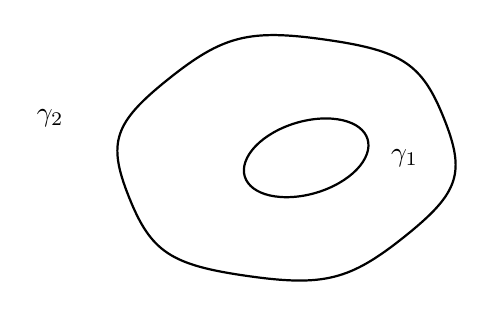
\begin{tikzpicture}
        % Draw the outer contour \gamma_2
        \draw[thick] plot [smooth cycle, tension=1] coordinates {(0,0) (2,0.5) (2.5,2) (1,3) (-1,2.5) (-1.5,1)};
        
        % Label the outer contour \gamma_2
        \node at (-2.5,2) {$\gamma_2$};
        
        % Draw the inner contour \gamma_1
        \draw[thick] plot [smooth cycle, tension=1] coordinates {(0.5,1) (1.5,1.5) (1,2) (0,1.5)};
        
        % Label the inner contour \gamma_1
        \node at (2,1.5) {$\gamma_1$};

        
        
    \end{tikzpicture}
    \caption{A simple closed contour \(\gamma_1\) contained in another simple closed contour \(\gamma_2\).}
\end{figure}

\begin{theorem}
    If \(z_0\) is a point interior to a positively-oriented simple closed contour \(\gamma\), then for any integer \(n \geq 1\),
    \[
        \oint_\gamma \frac{1}{(z - z_0)^n} \, dz = \begin{cases}
            \quad 0 & \text{ if } n \neq 1,\\
            \quad 2\pi i & \text{ if } n = 1.
        \end{cases}
    \]
\end{theorem}


\section{Consequences of Cauchy's theorem}

\begin{theorem}[Cauchy's integral]
    Let \(f\) be analytic in a simply connected domain \(\Omega\) and let
    \(\gamma\) be a positively-oriented simple closed contour that lies in
    \(\Omega\). Then if \(z_0\) is a point interior to \(\gamma\), then
    \[
        f(z_0) = \frac{1}{2\pi i} \oint_\gamma \frac{f(z)}{z - z_0} \, dz.
    \]
    \label{thm:cauchys-integral-formula}
\end{theorem}

\begin{example}
    Show that
    \[
        \oint_{\gamma} \frac{\exp z}{z - 1} \, dz = 2\pi i e,
    \]
    where \(\gamma\) is the circle of radius \(2\) centered at the origin.
\end{example}

\begin{theorem}[Cauchy's integral formula for derivatives]
    Let \(f\) be analytic in a simply connected domain \(\Omega\) and let
    \(\gamma\) be a positively-oriented simple closed contour that lies in
    \(\Omega\). Then if \(z_0\) is a point interior to \(\gamma\), then for any
    integer \(n \geq 0\),
    \[
        f^{(n)}(z_0) = \frac{n!}{2\pi i} \oint_\gamma \frac{f(z)}{(z - z_0)^{n+1}} \, dz.
    \]
    \label{thm:cauchys-integral-formula-nth-derivative}
\end{theorem}